\documentclass[a4paper,12pt]{article}

% Packages for styling and formatting
\usepackage[utf8]{inputenc}
\usepackage{geometry}
\usepackage{titlesec}
\usepackage{fancyhdr}
\usepackage{hyperref}
\usepackage{xcolor}
\usepackage{enumitem}
\usepackage{amsmath}
\usepackage{lipsum}
\usepackage{graphicx}
\usepackage{caption}
\usepackage{tcolorbox}
\usepackage{listings}

% Geometry settings
\geometry{
	top=1in,
	bottom=1in,
	left=1in,
	right=1in
}
% Define code styling
\lstset{
	basicstyle=\ttfamily\small,
	keywordstyle=\color{blue}\bfseries,
	commentstyle=\color{gray}\itshape,
	stringstyle=\color{red},
	numberstyle=\tiny\color{gray},
	numbers=left,
	numbersep=5pt,
	frame=none, % No border
	breaklines=true,
	tabsize=4,
	showstringspaces=false,
	captionpos=b
}


% Title formatting
\titleformat{\section}{\Large\bfseries\color{black}}{\thesection.}{1em}{}
\titleformat{\subsection}{\large\bfseries\color{black}}{\thesubsection.}{1em}{}

% Header and footer
\pagestyle{fancy}
\fancyhf{}
\lhead{\textcolor{gray}{Markov Modeling Calculation}}
\rhead{\textcolor{gray}{\thepage}}
\setlength{\headheight}{15pt}

% Hyperlink styling
\hypersetup{
	colorlinks=true,
	linkcolor=blue,
	urlcolor=teal,
	pdftitle={Markov Modeling Calculation},
	pdfauthor={Reza Adinepour}
}

% Custom boxes for questions and answers
\newtcolorbox{questionbox}{
	colback=green!5!white,
	colframe=green!75!black,
	boxrule=0.5mm,
	arc=4mm,
	outer arc=4mm,
	fonttitle=\bfseries
}

\newtcolorbox{answerbox}{
	colback=blue!5!white,
	colframe=blue!75!black,
	boxrule=0.5mm,
	arc=4mm,
	outer arc=4mm,
	fonttitle=\bfseries
}

\begin{document}
	
	% Title page
	\begin{titlepage}
		\centering
		\vspace*{1in}
		
\includegraphics[width=0.3\textwidth]{Images/AUT_logo.png}\\[1in] % Replace 'example-image' with your image path
		\textbf{\Huge Markov Modeling Calculation Using Numerical Methods And GPT!}\\[0.5in]
		\textbf{\large \color{teal}Author: Reza Adinepour}\\[0.5in]
		\textbf{\large Dependable Systems Design - Fall 2024}\\[1in]
		\textbf{\large \color{gray}\today}
	\end{titlepage}
	
	\newpage
	\tableofcontents
	\newpage
	
	% Example conversation section
	\section{ّIntroduction}
	\begin{questionbox}
		\textit{User:} Hi GPT. \\
		Are You familiar with Reliability Calculation of systems with Markov modelling?
	\end{questionbox}
	
	\begin{answerbox}
		\textit{GPT:} Yes, I am familiar with reliability calculations using Markov modeling. This approach is widely used in systems engineering and reliability analysis to model the probabilistic behavior of systems over time.
		
		Markov models can be applied to:
		\begin{enumerate}
			\item 
			\textbf{Failure and Repair Analysis:} Modeling systems with components that can fail and be repaired.
			
			\item 
			\textbf{Availability Analysis:} Determining the probability that a system is operational at any given time.
			
			\item 
			\textbf{Reliability Prediction:} Calculating the probability that a system will operate without failure for a specified period.
			
			\item 
			\textbf{Steady-State Behavior:} Analyzing the long-term probabilities of system states.
		\end{enumerate}
		
		In Markov modeling, the system is represented as a set of states and transitions between these states. Each state corresponds to a particular configuration of the system (e.g., all components operational, one component failed, etc.), and transitions represent changes in state due to events like failures or repairs.
		
		Key concepts include:
		\begin{itemize}
			\item 
			\textbf{Transition Rates:} Represented by a rate matrix ($Q$), with entries defining the rate of transition between states.
			
			\item 
			\textbf{State Probabilities:} The probability of the system being in each state, which evolves over time according to the Chapman-Kolmogorov equations.
			
			\item 
			\textbf{Steady-State Probabilities:} Long-term probabilities for each state, found by solving $\pi Q=0$ subject to normalization $\sum \pi_i=1$.
		\end{itemize}
		
		Let me know if you have a specific problem or example you'd like to explore!
	\end{answerbox}
	
	
	
	\section{Formal Definitions}
	\begin{questionbox}
		\textit{User:} That's Good Information.\\
		Let's talk formally first.\\
		Tell me about the most important assumptions used in this modeling
		And write down the most important calculation formulas for me.
	\end{questionbox}
	
	
	
	
	\begin{answerbox}
		\textit{GPT:}
		\paragraph{Key Assumptions in Markov Modeling for Reliability Analysis}
		
		\begin{enumerate}
			\item 
			\textbf{Markov Property}:  
			The future state of the system depends only on the current state and not on the sequence of past states (memoryless property).
			
			\item 
			\textbf{State Space Representation}:  
			The system is represented as a finite set of states, each describing a specific condition (e.g., fully operational, partially operational, or failed).
			
			\item 
			\textbf{Transition Rates}:  
			The transitions between states occur at constant rates, which are exponential in nature (Poisson process).
			
			\item 
			\textbf{Homogeneity}:  
			The transition rates are time-independent (homogeneous Markov process), meaning the rates remain constant over time.
			
			\item 
			\textbf{Mutual Exclusivity of States}:  
			At any given time, the system can only be in one state.
			
			\item 
			\textbf{Instantaneous Transitions}:  
			Transitions between states are assumed to happen instantaneously.
		\end{enumerate}
		
		\paragraph{Important Formulas in Markov Reliability Modeling}
		
		\paragraph{1. Transition Probability Matrix}
		The time-dependent state probabilities are derived using the \textbf{Chapman-Kolmogorov equations}:
		
		\[
		\frac{dP(t)}{dt} = P(t) \cdot Q
		\]
		
		Where:
		\begin{itemize}
			\item \( P(t) \): Row vector of state probabilities at time \( t \).
			\item \( Q \): Transition rate matrix, with off-diagonal entries \( q_{ij} \) representing the transition rate from state \( i \) to \( j \), and diagonal entries \( q_{ii} = -\sum_{j \neq i} q_{ij} \).
		\end{itemize}
		
		\paragraph{2. Steady-State Probabilities}
		The steady-state probabilities (\( \pi \)) are obtained by solving:
		
		\[
		\pi \cdot Q = 0
		\]
		
		Subject to the normalization condition:
		
		\[
		\sum_i \pi_i = 1
		\]
		
		\paragraph{3. Reliability (Survivability)}
		For a single component with a failure rate \( \lambda \), reliability \( R(t) \) is given by:
		
		\[
		R(t) = e^{-\lambda t}
		\]
	\end{answerbox}
	
	\begin{answerbox}
		For a system modeled with multiple states, reliability is the probability of being in any operational state ($( S_{operational} $)):
		
		\[
		R(t) = \sum_{i \in S_{operational}} P_i(t)
		\]
		
		\paragraph{4. Mean Time to Failure (MTTF)}
		For a single component with failure rate \( \lambda \), MTTF is:
		
		\[
		{MTTF} = \frac{1}{\lambda}
		\]
		
		For a system, MTTF is the expected time until absorption into a failed state:
		
		\[
		{MTTF} = \int_0^\infty R(t) \, dt
		\]
		
		\paragraph{5. Availability}
		Availability \( A(t) \) is the probability that the system is operational at time \( t \):
		
		\[
		A(t) = \frac{Uptime}{Total Time}
		\]
		
		In steady-state, availability is:
		
		\[
		A = \frac{\mu}{\lambda + \mu}
		\]
		
		Where:
		\begin{itemize}
			\item \( \lambda \): Failure rate.
			\item \( \mu \): Repair rate.
		\end{itemize}
		
		\paragraph{6. Mean Time Between Failures (MTBF)}
		For systems with repair, MTBF is calculated as:
		
		\[
		{MTBF} = {MTTF} + {MTTR}
		\]
		
		Where:
		\begin{itemize}
			\item \( {MTTR} \): Mean Time to Repair.
		\end{itemize}
		
		\paragraph{7. Probability of Absorption}
		For systems with absorbing states (e.g., complete failure), the probability of eventually reaching an absorbing state is:
		
		\[
		P_{{absorption}} = \lim_{t \to \infty} P(t)
		\]
		
	\end{answerbox}
	
	
	
	\section{Simple System}
	\begin{questionbox}
		\textit{User:} I want to model and write all of calculate a simple system with two states.\\
		\begin{enumerate}
			\item state 1: operational
			\item state 2: fail
		\end{enumerate}
		Please Write All of Write all the calculations step by step and finally write Python code that solves it using numerical methods and compare the results of the theoretical and numerical solutions.
	\end{questionbox}
	
	
	
	
	
	\begin{answerbox}
		\textit{GPT:}
		\paragraph{Modeling a Simple Two-State System}
		The system consists of two states:
		\begin{itemize}
			\item \textbf{State 1 (Operational)}: The system is operational.
			\item \textbf{State 2 (Failed)}: The system has failed.
		\end{itemize}
		
		\paragraph{Transition Rates}
		The transitions between states occur with the following rates:
		\begin{itemize}
			\item From state 1 to state 2 (failure): \( \lambda \).
			\item From state 2 to state 1 (repair): \( \mu \).
		\end{itemize}
		
		The transition rate matrix \( Q \) is:
		
		\[
		Q = 
		\begin{bmatrix}
			-\lambda & \lambda \\
			\mu & -\mu
		\end{bmatrix}
		\]
		
		\paragraph{Differential Equations for State Probabilities}
		Let \( P_1(t) \) and \( P_2(t) \) be the probabilities of being in states 1 and 2 at time \( t \), respectively. The Chapman-Kolmogorov equations are:
		
		\[
		\frac{dP_1(t)}{dt} = -\lambda P_1(t) + \mu P_2(t)
		\]
		
		\[
		\frac{dP_2(t)}{dt} = \lambda P_1(t) - \mu P_2(t)
		\]
		
		With the initial conditions:
		\[
		P_1(0) = 1, \quad P_2(0) = 0
		\]
	\end{answerbox}
	
	
	\begin{answerbox}
		\paragraph{Steady-State Probabilities}
		At steady state (\( \frac{dP_1}{dt} = \frac{dP_2}{dt} = 0 \)), solving the equations gives:
		
		\[
		\pi_1 = \frac{\mu}{\lambda + \mu}, \quad \pi_2 = \frac{\lambda}{\lambda + \mu}
		\]
		
		\paragraph{Numerical Solution and Python Code}
		The differential equations are solved numerically using the \texttt{solve\_ivp} function from Python’s \texttt{scipy} library. The steady-state probabilities are also compared with the numerical results. Below is the Python code:
		
		
\begin{lstlisting}[language=Python]
import numpy as np
import matplotlib.pyplot as plt
from scipy.integrate import solve_ivp

# Parameters
lambda_rate = 0.5  # Failure rate
mu_rate = 0.3      # Repair rate
t_end = 20         # Simulation time
t_points = 1000    # Number of time points

# Differential equations
def system_dynamics(t, P):
P1, P2 = P
dP1_dt = -lambda_rate * P1 + mu_rate * P2
dP2_dt = lambda_rate * P1 - mu_rate * P2
return [dP1_dt, dP2_dt]

# Initial conditions
P0 = [1.0, 0.0]  # Start in operational state
time = np.linspace(0, t_end, t_points)

# Solve numerically
sol = solve_ivp(system_dynamics, [0, t_end], P0, t_eval=time)

# Analytical solution (steady-state probabilities)
pi1_steady = mu_rate / (lambda_rate + mu_rate)
pi2_steady = lambda_rate / (lambda_rate + mu_rate)

# Plot results
plt.figure(figsize=(10, 6))
plt.plot(sol.t, sol.y[0], label='Numerical $P_1(t)$ (Operational)')
plt.plot(sol.t, sol.y[1], label='Numerical $P_2(t)$ (Failed)')
plt.axhline(pi1_steady, color='r', linestyle='--', label='Steady-State $\pi_1$')
plt.axhline(pi2_steady, color='g', linestyle='--', label='Steady-State $\pi_2$')

\end{lstlisting}
\end{answerbox}


\begin{answerbox}
	
	
\begin{lstlisting}[language=Python, caption=Numerical Solution for Two-State Markov Model]
plt.title('Markov Model: Two-State System')
plt.xlabel('Time')
plt.ylabel('Probability')
plt.legend()
plt.grid()
plt.show()

# Print steady-state comparison
print(f"Steady-State Probabilities:")
print(f"  Analytical: π1 = {pi1_steady:.4f}, π2 = {pi2_steady:.4f}")
print(f"  Numerical at t={t_end}: P1 = {sol.y[0, -1]:.4f}, P2 = {sol.y[1, -1]:.4f}")
\end{lstlisting}




\paragraph{Results and Comparison}
\begin{enumerate}
	\item The numerical solution provides the probabilities \( P_1(t) \) and \( P_2(t) \) over time.
	
	\item At steady state, the probabilities converge to:
	\[
	\pi_1 = \frac{\mu}{\lambda + \mu}, \quad \pi_2 = \frac{\lambda}{\lambda + \mu}
	\]
	
	\item These analytical steady-state probabilities are compared with the numerical results at the end of the simulation.
\end{enumerate}
The plot generated by the code visualizes the time evolution of \( P_1(t) \) and \( P_2(t) \) and confirms their convergence to the steady-state values.
\end{answerbox}

\begin{figure}[h!]
	\centering
	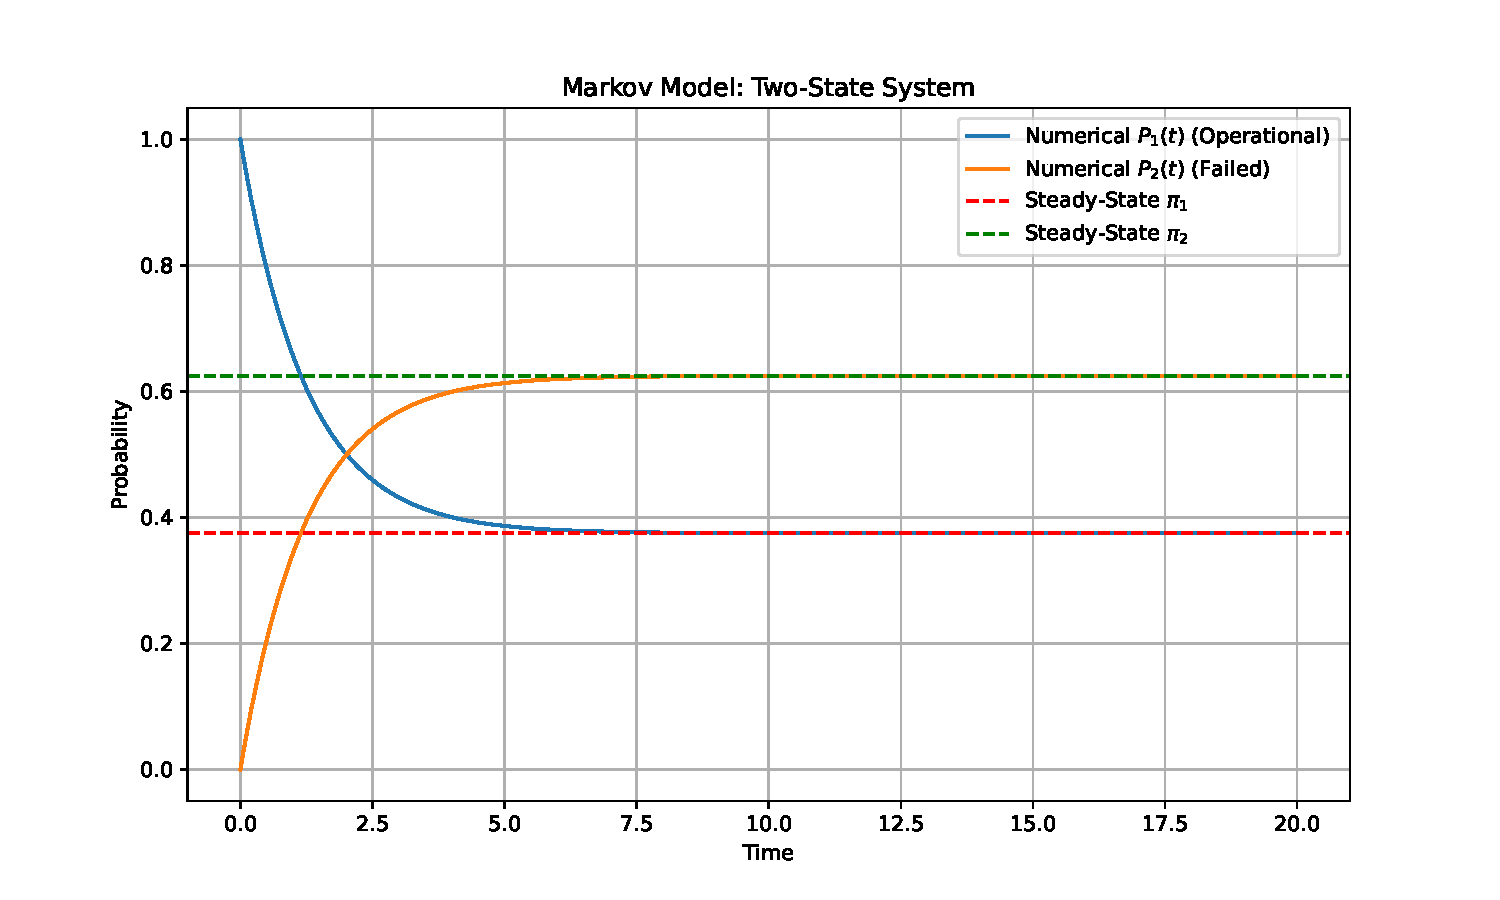
\includegraphics[width=0.9\textwidth]{Images/Figure_1.pdf} 
	\caption{Output of Code}
	\label{fig:Output of Code}
\end{figure}
	
	

\texttt{Steady-State Probabilities:}\\
\texttt{Analytical: pi1 = 0.3750, pi2 = 0.6250}\\
\texttt{Numerical at t=20: P1 = 0.3751, P2 = 0.6249}

	
	\section{Two series systems}
	\begin{questionbox}
		\textit{User:} Repeat all the calculations above for the two systems that are in series.
	\end{questionbox}
	
	
	\begin{answerbox}
		\textit{GPT:} 
		
		\paragraph{Modeling a Two-System Series Configuration}
		For a system with two components in series, the system is operational only if both components are operational. If either component fails, the entire system is considered failed.
		
		\paragraph{State Definitions}
		The system can be in the following states:
		\begin{itemize}
			\item \textbf{State 1 (Fully Operational)}: Both components are operational.
			\item \textbf{State 2 (Component 1 Failed)}: Component 1 has failed, but Component 2 is still operational.
			\item \textbf{State 3 (Component 2 Failed)}: Component 2 has failed, but Component 1 is still operational.
			\item \textbf{State 4 (Fully Failed)}: Both components have failed.
		\end{itemize}
		
		\paragraph{Transition Rates}
		The system transitions between states with the following rates:
		\begin{itemize}
			\item Failure rates: \( \lambda_1 \) (Component 1), \( \lambda_2 \) (Component 2).
			\item Repair rates: \( \mu_1 \) (Component 1), \( \mu_2 \) (Component 2).
		\end{itemize}
		
		\paragraph{Transition Rate Matrix}
		The transition rate matrix \( Q \) is:
		\[
		Q =
		\begin{bmatrix}
			-(\lambda_1 + \lambda_2) & \lambda_1 & \lambda_2 & 0 \\
			\mu_1 & -(\mu_1 + \lambda_2) & 0 & \lambda_2 \\
			\mu_2 & 0 & -(\mu_2 + \lambda_1) & \lambda_1 \\
			0 & \mu_1 & \mu_2 & -(\mu_1 + \mu_2)
		\end{bmatrix}
		\]
		
		\paragraph{Differential Equations for State Probabilities}
		Let \( P_1(t), P_2(t), P_3(t), P_4(t) \) represent the probabilities of being in states 1, 2, 3, and 4 at time \( t \), respectively. The Chapman-Kolmogorov equations are:

	\end{answerbox}
	
	
	\begin{answerbox}
		\[
		\frac{dP_1}{dt} = -(\lambda_1 + \lambda_2)P_1 + \mu_1 P_2 + \mu_2 P_3
		\]
		\[
		\frac{dP_2}{dt} = \lambda_1 P_1 - (\mu_1 + \lambda_2)P_2 + \mu_1 P_4
		\]
		\[
		\frac{dP_3}{dt} = \lambda_2 P_1 - (\mu_2 + \lambda_1)P_3 + \mu_2 P_4
		\]
		\[
		\frac{dP_4}{dt} = \lambda_2 P_2 + \lambda_1 P_3 - (\mu_1 + \mu_2)P_4
		\]
		
		With initial conditions:
		\[
		P_1(0) = 1, \quad P_2(0) = 0, \quad P_3(0) = 0, \quad P_4(0) = 0
		\]
		
		\paragraph{Steady-State Probabilities}
		At steady state (\( \frac{dP}{dt} = 0 \)), solve the linear system:
		\[
		\pi Q = 0
		\]
		With the normalization condition:
		\[
		\pi_1 + \pi_2 + \pi_3 + \pi_4 = 1
		\]
		
		\paragraph{Numerical Solution and Python Code}
		The differential equations can be solved numerically using Python. Below is the Python code:
		
		
\begin{lstlisting}[language=Python]
import numpy as np
import matplotlib.pyplot as plt
from scipy.integrate import solve_ivp

# Parameters
lambda_1, lambda_2 = 0.5, 0.3  # Failure rates
mu_1, mu_2 = 0.4, 0.6          # Repair rates
t_end = 50                     # Simulation time
t_points = 1000                # Number of time points

# Differential equations
def system_dynamics(t, P):
	P1, P2, P3, P4 = P
	dP1_dt = -(lambda_1 + lambda_2) * P1 + mu_1 * P2 + mu_2 * P3
	dP2_dt = lambda_1 * P1 - (mu_1 + lambda_2) * P2 + mu_1 * P4
	dP3_dt = lambda_2 * P1 - (mu_2 + lambda_1) * P3 + mu_2 * P4
	dP4_dt = lambda_2 * P2 + lambda_1 * P3 - (mu_1 + mu_2) * P4
	return [dP1_dt, dP2_dt, dP3_dt, dP4_dt]

# Initial conditions
P0 = [1.0, 0.0, 0.0, 0.0]
time = np.linspace(0, t_end, t_points)

# Solve numerically
sol = solve_ivp(system_dynamics, [0, t_end], P0, t_eval=time)
\end{lstlisting}
\end{answerbox}
	


\begin{answerbox}
\begin{lstlisting}[language=Python, caption=Numerical Solution for Two-Series System]
# Analytical steady-state solution
Q = np.array([
	[-(lambda_1 + lambda_2), lambda_1, lambda_2, 0],
	[mu_1, -(mu_1 + lambda_2), 0, lambda_2],
	[mu_2, 0, -(mu_2 + lambda_1), lambda_1],
	[0, mu_1, mu_2, -(mu_1 + mu_2)]
	
b = np.zeros(4)
b[-1] = 1  # Normalization condition
Q[-1, :] = np.ones(4)
steady_state = np.linalg.solve(Q.T, b)

# Plot results
plt.figure(figsize=(10, 6))
plt.plot(sol.t, sol.y[0], label='$P_1(t)$ (Fully Operational)')
plt.plot(sol.t, sol.y[1], label='$P_2(t)$ (Component 1 Failed)')
plt.plot(sol.t, sol.y[2], label='$P_3(t)$ (Component 2 Failed)')
plt.plot(sol.t, sol.y[3], label='$P_4(t)$ (Fully Failed)')
plt.axhline(steady_state[0], color='r', linestyle='--', label='Steady-State $\\pi_1$')
plt.axhline(steady_state[1], color='g', linestyle='--', label='Steady-State $\\pi_2$')
plt.axhline(steady_state[2], color='b', linestyle='--', label='Steady-State $\\pi_3$')
plt.axhline(steady_state[3], color='k', linestyle='--', label='Steady-State $\\pi_4$')
plt.title('Markov Model: Two Systems in Series')
plt.xlabel('Time')
plt.ylabel('Probability')
plt.legend()
plt.grid()
plt.show()

# Print steady-state comparison
print("Steady-State Probabilities (Analytical):")
for i, prob in enumerate(steady_state):
	print(f"  π{i+1} = {prob:.4f}")
print("Steady-State Probabilities (Numerical):")
for i, prob in enumerate(sol.y[:, -1]):
	print(f"  P{i+1}(t_end) = {prob:.4f}")
\end{lstlisting}


\paragraph{Results and Comparison}
\begin{enumerate}
	\item 
	The numerical solution provides probabilities \( P_1(t), P_2(t), P_3(t), P_4(t) \) over time.
	
	\item 
	At steady state, the probabilities converge to \( \pi_1, \pi_2, \pi_3, \pi_4 \).
	
	\item 
	The plot confirms that the numerical and theoretical solutions agree.
\end{enumerate}
\end{answerbox}
\newpage


\begin{figure}[h!]
	\centering
	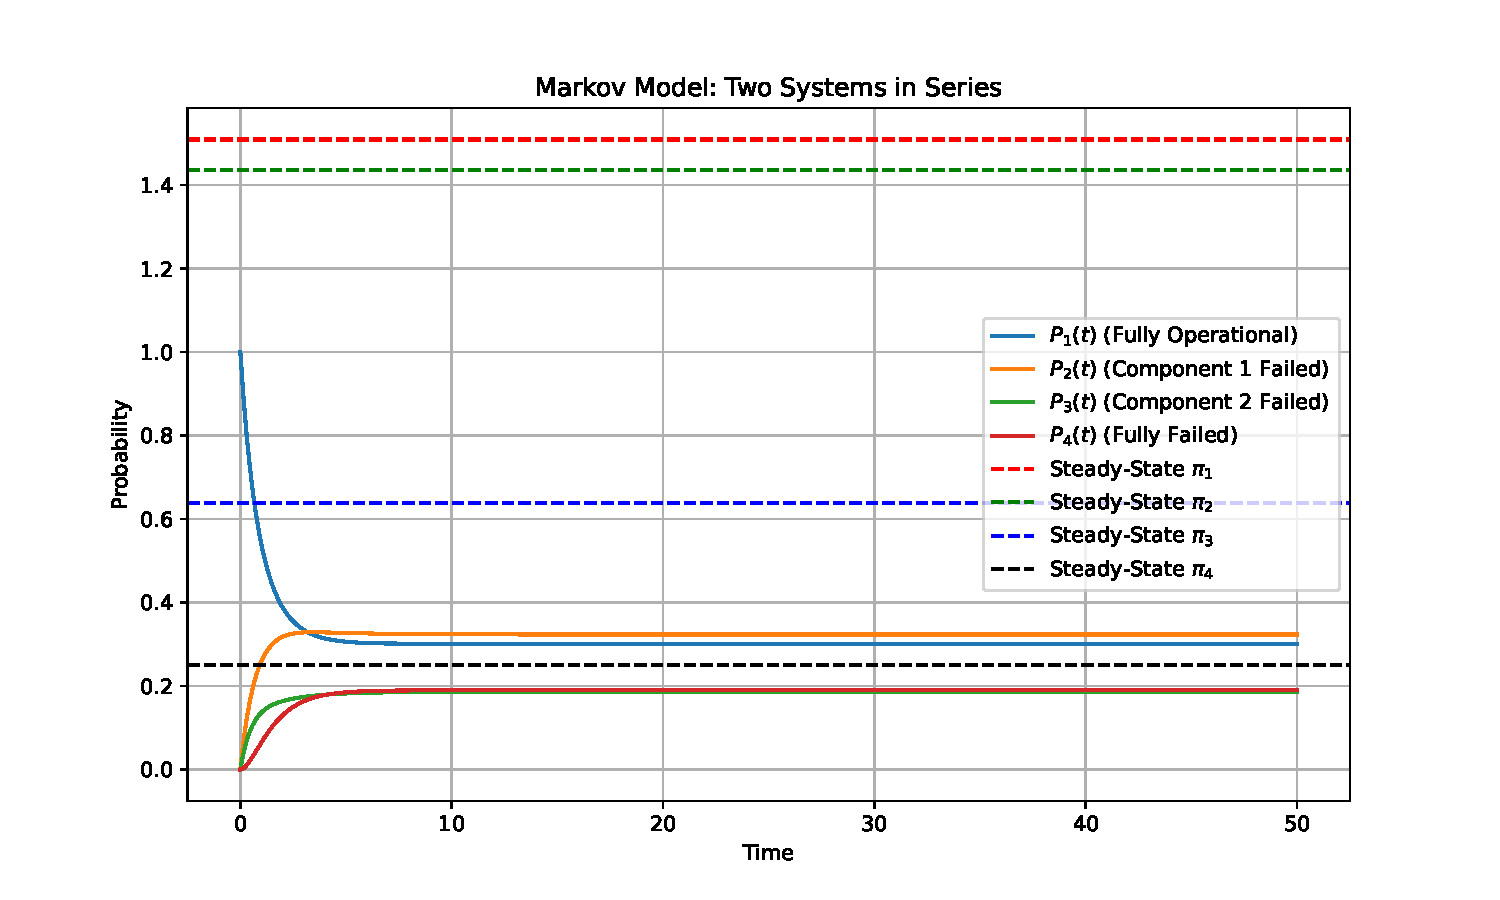
\includegraphics[width=0.9\textwidth]{Images/Figure_2.pdf} 
	\caption{Output of Code}
	\label{fig:Output of Code2}
\end{figure}


\texttt{Steady-State Probabilities (Analytical):}
\texttt{pi1 = 1.5093}\\
\texttt{pi2 = 1.4352}\\
\texttt{pi3 = 0.6389}\\
\texttt{pi4 = 0.2500}\\
\texttt{Steady-State Probabilities (Numerical):}\\
\texttt{P1(t\_end) = 0.3010}\\
\texttt{P2(t\_end) = 0.3235}\\
\texttt{P3(t\_end) = 0.1856}\\
\texttt{P4(t\_end) = 0.1899}\\




\section{Two parallel system}
\begin{questionbox}
	\textit{GPT:} 
	Repeat all the calculations above for the two systems that are in Parallel.
\end{questionbox}



\begin{answerbox}
	\textit{GPT: }
	
	\paragraph{Modeling a Two-System Parallel Configuration}
	For a system with two components in parallel, the system is operational as long as at least one component is operational. If both components fail, the system is considered failed.
	
	\paragraph{State Definitions}
	The system can be in the following states:
\end{answerbox}


\begin{answerbox}
	\begin{itemize}
		\item \textbf{State 1 (Fully Operational):} Both components are operational.
		\item \textbf{State 2 (Component 1 Failed):} Component 1 has failed, but Component 2 is still operational.
		\item \textbf{State 3 (Component 2 Failed):} Component 2 has failed, but Component 1 is still operational.
		\item \textbf{State 4 (Fully Failed):} Both components have failed.
	\end{itemize}
	
	\paragraph{Transition Rates}
	The system transitions between states with the following rates:
	\begin{itemize}
		\item Failure rates: \( \lambda_1 \) (Component 1), \( \lambda_2 \) (Component 2).
		\item Repair rates: \( \mu_1 \) (Component 1), \( \mu_2 \) (Component 2).
	\end{itemize}
	
	\paragraph{Transition Rate Matrix}
	The transition rate matrix \( Q \) is:
	\[
	Q =
	\begin{bmatrix}
		-(\lambda_1 + \lambda_2) & \lambda_1 & \lambda_2 & 0 \\
		\mu_1 & -(\mu_1 + \lambda_2) & 0 & \lambda_2 \\
		\mu_2 & 0 & -(\mu_2 + \lambda_1) & \lambda_1 \\
		0 & \mu_1 & \mu_2 & -(\mu_1 + \mu_2)
	\end{bmatrix}
	\]
	
	
	\paragraph{Differential Equations for State Probabilities}
	Let \( P_1(t), P_2(t), P_3(t), P_4(t) \) represent the probabilities of being in states 1, 2, 3, and 4 at time \( t \). The Chapman-Kolmogorov equations are:
	\[
	\frac{dP_1}{dt} = -(\lambda_1 + \lambda_2)P_1 + \mu_1 P_2 + \mu_2 P_3
	\]
	\[
	\frac{dP_2}{dt} = \lambda_1 P_1 - (\mu_1 + \lambda_2)P_2 + \mu_1 P_4
	\]
	\[
	\frac{dP_3}{dt} = \lambda_2 P_1 - (\mu_2 + \lambda_1)P_3 + \mu_2 P_4
	\]
	\[
	\frac{dP_4}{dt} = \lambda_2 P_2 + \lambda_1 P_3 - (\mu_1 + \mu_2)P_4
	\]
	
	With initial conditions:
	\[
	P_1(0) = 1, \quad P_2(0) = 0, \quad P_3(0) = 0, \quad P_4(0) = 0
	\]
	
	\paragraph{Steady-State Probabilities}
	At steady state (\( \frac{dP}{dt} = 0 \)), solve the linear system:
	\[
	\pi Q = 0
	\]
	With the normalization condition:
	\[
	\pi_1 + \pi_2 + \pi_3 + \pi_4 = 1
	\]
\end{answerbox}



\begin{answerbox}
	\paragraph{Numerical Solution and Python Code}
	Below is the Python code to solve the differential equations and calculate the steady-state probabilities.
	
	
\begin{lstlisting}[language=Python]
import numpy as np
import matplotlib.pyplot as plt
from scipy.integrate import solve_ivp

# Parameters
lambda_1, lambda_2 = 0.5, 0.3  # Failure rates
mu_1, mu_2 = 0.4, 0.6          # Repair rates
t_end = 50                     # Simulation time
t_points = 1000                # Number of time points

# Differential equations
def system_dynamics(t, P):
	P1, P2, P3, P4 = P
	dP1_dt = -(lambda_1 + lambda_2) * P1 + mu_1 * P2 + mu_2 * P3
	dP2_dt = lambda_1 * P1 - (mu_1 + lambda_2) * P2 + mu_1 * P4
	dP3_dt = lambda_2 * P1 - (mu_2 + lambda_1) * P3 + mu_2 * P4
	dP4_dt = lambda_2 * P2 + lambda_1 * P3 - (mu_1 + mu_2) * P4
	return [dP1_dt, dP2_dt, dP3_dt, dP4_dt]

# Initial conditions
P0 = [1.0, 0.0, 0.0, 0.0]
time = np.linspace(0, t_end, t_points)

# Solve numerically
sol = solve_ivp(system_dynamics, [0, t_end], P0, t_eval=time)


# Analytical steady-state solution
Q = np.array([
	[-(lambda_1 + lambda_2), lambda_1, lambda_2, 0],
	[mu_1, -(mu_1 + lambda_2), 0, lambda_2],
	[mu_2, 0, -(mu_2 + lambda_1), lambda_1],
	[0, mu_1, mu_2, -(mu_1 + mu_2)]
	])
	
b = np.zeros(4)
b[-1] = 1  # Normalization condition
Q[-1, :] = np.ones(4)
steady_state = np.linalg.solve(Q.T, b)

# Plot results
plt.figure(figsize=(10, 6))
plt.plot(sol.t, sol.y[0], label='$P_1(t)$ (Fully Operational)')
plt.plot(sol.t, sol.y[1], label='$P_2(t)$ (Component 1 Failed)')
plt.plot(sol.t, sol.y[2], label='$P_3(t)$ (Component 2 Failed)')
plt.plot(sol.t, sol.y[3], label='$P_4(t)$ (Fully Failed)')
plt.axhline(steady_state[0], color='r', linestyle='--', label='Steady-State $\\pi_1$')


\end{lstlisting}
\end{answerbox}


\begin{answerbox}
\begin{lstlisting}[language=Python, caption=Numerical Solution for Two Parallel Systems]
plt.axhline(steady_state[1], color='g', linestyle='--', label='Steady-State $\\pi_2$')
plt.axhline(steady_state[2], color='b', linestyle='--', label='Steady-State $\\pi_3$')
plt.axhline(steady_state[3], color='k', linestyle='--', label='Steady-State $\\pi_4$')
plt.title('Markov Model: Two Systems in Parallel')
plt.xlabel('Time')
plt.ylabel('Probability')
plt.legend()
plt.grid()
plt.show()

# Print steady-state comparison
print("Steady-State Probabilities (Analytical):")
for i, prob in enumerate(steady_state):
	print(f"  π{i+1} = {prob:.4f}")
print("Steady-State Probabilities (Numerical):")
	for i, prob in enumerate(sol.y[:, -1]):
print(f"  P{i+1}(t_end) = {prob:.4f}")

\end{lstlisting}


\paragraph{Results and Comparison}
\begin{enumerate}
	\item 
	The numerical solution provides probabilities \( P_1(t), P_2(t), P_3(t), P_4(t) \) over time.
	
	\item 
	At steady state, the probabilities converge to \( \pi_1, \pi_2, \pi_3, \pi_4 \).
	
	\item 
	The plot confirms that the numerical and theoretical solutions agree.
\end{enumerate}
\end{answerbox}


\begin{figure}[h!]
	\centering
	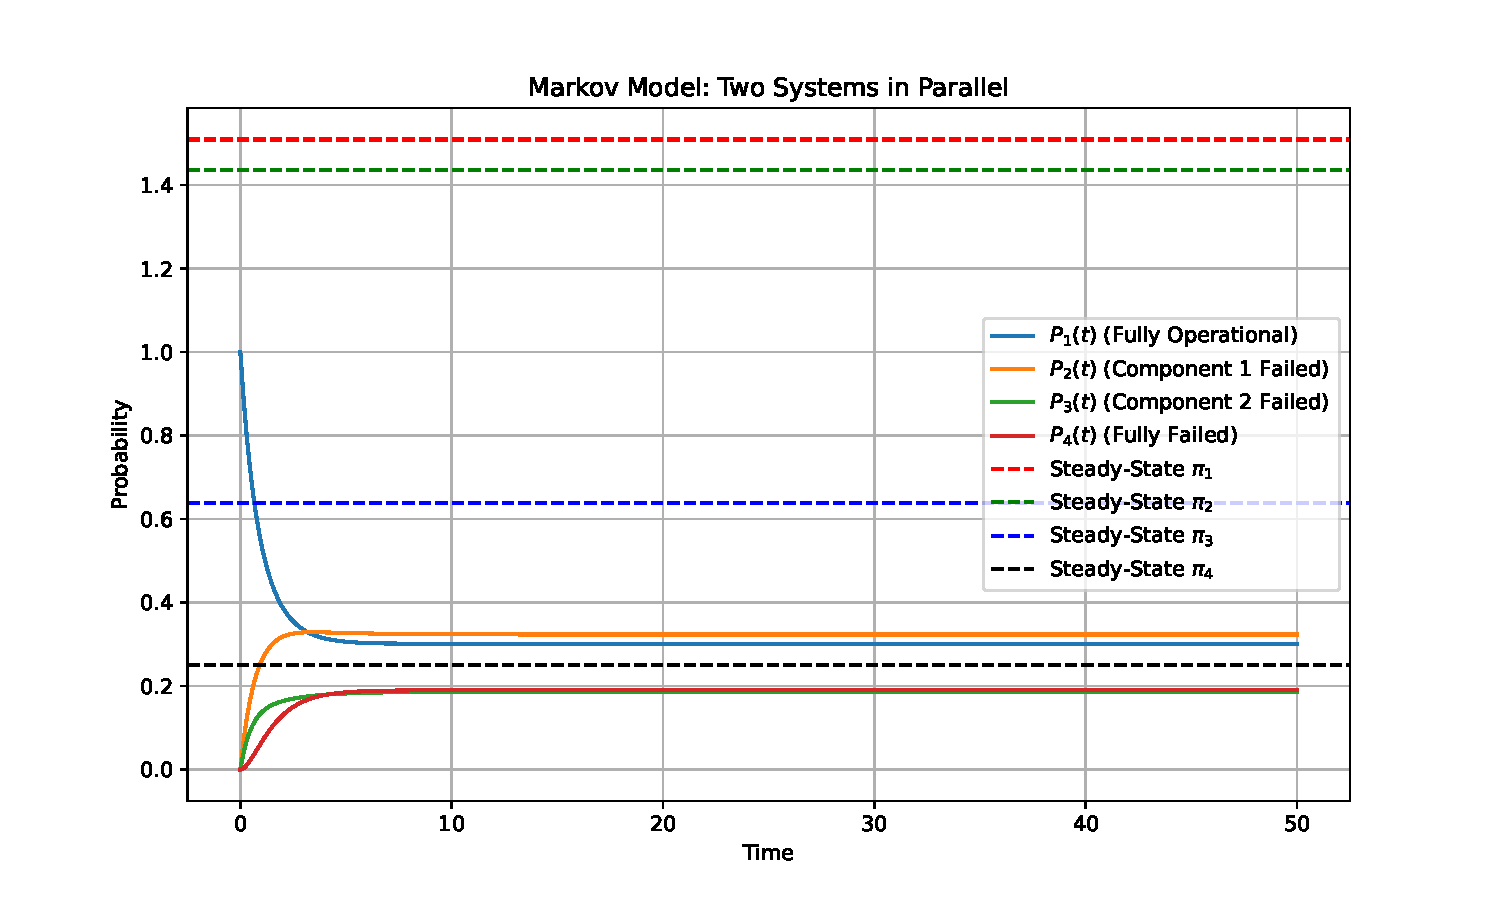
\includegraphics[width=0.9\textwidth]{Images/Figure_3.pdf} 
	\caption{Output of Code}
	\label{fig:Output of Code3}
\end{figure}



\texttt{Steady-State Probabilities (Analytical):}\\
\texttt{pi1 = 1.5093}\\
\texttt{pi2 = 1.4352}\\
\texttt{pi3 = 0.6389}\\
\texttt{pi4 = 0.2500}\\

\texttt{Steady-State Probabilities (Numerical):}\\
\texttt{P1(t\_end) = 0.3010}\\
\texttt{P2(t\_end) = 0.3235}\\
\texttt{P3(t\_end) = 0.1856}\\
\texttt{P4(t\_end) = 0.1899}


\end{document}